\chapter{Quickstart}
\label{chap:quickstart}
\index{quickstart}

This chapter demonstrates how to get started with \dolfin{}, including
downloading and installing the latest version of \dolfin{}, and solving
Poisson's equation. These topics are discussed in more detail
elsewhere in this manual. In particular, see
Appendix~\ref{app:installation} for detailed installation instructions
and Chapter~\ref{sec:pde} for a detailed discussion of how to solve
partial differential equations with \dolfin{}.

%------------------------------------------------------------------------------
\section{Downloading and installing \dolfin{}}
\index{downloading}
\index{installation}

The latest version of \dolfin{} can be found on the \fenics{} web page:
\begin{code}
http://www.fenics.org/
\end{code}
The following commands illustrate the installation process, assuming
that you have downloaded release x.y.z of \dolfin{}:
\begin{code}
# tar zxfv dolfin-x.y.z.tar.gz
# cd dolfin-x.y.z
# ./configure
# make
# sudo make install
\end{code}

Since \dolfin{} depends on a number of other packages, you may also
need to download and install those packages before you can compile
\dolfin{}.  (See Appendix~\ref{app:installation} for detailed
instructions.)

%------------------------------------------------------------------------------
\section{Solving Poisson's equation with \dolfin{}}
\index{Poisson's equation}

Let's say that we want to solve Poisson's equation on the unit square
$\Omega = (0,1) \times (0,1)$ with homogeneous Dirichlet boundary
conditions on the boundary $\Gamma_0 = \{(x, y) \in \partial \Omega : x = 0\}$,
the Neumann boundary condition $\partial_n u = g$ 
with $g(x, y) = 25 \sin(5\pi y)$
on the boundary $\Gamma_1 = \{(x, y) \in \partial \Omega : x = 1\}$,
homogeneous Neumann boundary conditions on the remaining part of the boundary
and right-hand side given by $f(x, y) = 500 \exp(-((x-0.5)^2 +
(y-0.5)^2)/0.02)$:
\begin{eqnarray} \label{eq:poisson,quickstart}
  - \Delta u(x, y) &=& f(x, y), \quad
  x \in \Omega = (0,1) \times (0,1), \\
  u(x, y) &=& 0, \quad
  (x, y) \in \Gamma_0 = \{(x, y) \in \partial \Omega : x = 0\}, \\
  \partial_n u(x, y) &=& 1, \quad
  (x, y) \in \Gamma_1 = \{(x, y) \in \partial \Omega : x = 1\}, \\
  \partial_n u(x, y) &=& 0, \quad
  (x, y) \in \partial \Omega \setminus (\Gamma_0 \cup \Gamma_1).
\end{eqnarray}

% FIXME: Explain this better

To solve a partial differential equation with \dolfin{}, it must first
be rewritten in \emph{variational form}.  The (discrete) variational
formulation of Poisson's equation reads: Find $u_h \in V_h$ such that
\begin{equation} \label{eq:varform}
  a(v, u_h) = L(v) \quad \forall v\in \hat{V}_h, 
\end{equation}
with $(\hat{V}_h, V_h)$ a pair of suitable discrete function spaces
(the test and trial spaces). The bilinear form $a : \hat{V}_h \times V_h
\rightarrow \R$ is given by
\begin{equation}
  a(v, u_h) = \int_{\Omega} \nabla v \cdot \nabla u_h \dx
\end{equation}
and the linear form $L : \hat{V}_h \rightarrow \R$ is given by
\begin{equation}
  L(v) = \int_{\Omega} v f \dx + \int_{\partial \Omega} v g \ds,
\end{equation}
where $g = \partial_n u$ is the Neumann boundary condition.

\subsection{Setting up the variational formulation}
\index{ffc}

The variational formulation (\ref{eq:varform}) must be given to
\dolfin{} as a pair of bilinear and linear forms $(a, L)$ using the
form compiler \ffc{}. This is done by entering the definition of
the forms in a text file with extension \texttt{.form},
e.g. \texttt{Poisson.form}, as follows:
\begin{code}
element = FiniteElement("Lagrange", "triangle", 1)

v = TestFunction(element)
u = TrialFunction(element)
f = Function(element)
g = Function(element)

a = dot(grad(v), grad(u))*dx
L = v*f*dx + v*g*ds
\end{code}

The example is given here for piecewise linear finite elements in two
dimensions, but other choices are available, including arbitrary order
Lagrange elements in two and three dimensions.

To compile the pair of forms $(a, L)$, now call the form compiler on
the command-line as follows:
\begin{code}
# ffc -l dolfin Poisson.form
\end{code}
This generates the file \texttt{Poisson.h} which implements the forms
in C++ for inclusion in your \dolfin{} program.

\subsection{Writing the solver}

Having compiled the variational formulation (\ref{eq:varform})
with \ffc{}, it is now easy to implement a solver for Poisson's
equation. We first discuss the implementation line by line and then
present the complete program. The source code for this example is
available in the directory \texttt{src/demo/pde/poisson/} of the \dolfin{}
source tree.

At the beginning of our C++ program, which we write in a text file
named \texttt{main.cpp}, we must first include the header file
\texttt{dolfin.h}, which gives our program access to the \dolfin{}
class library. In addition, we include the header file
\texttt{Poisson.h} generated by the form compiler. Since all classes
in the \dolfin{} class library are defined within the namespace
\texttt{dolfin}, we also specify that we want to work within this
namespace:
\begin{code}
#include <dolfin.h>
#include "Poisson.h"
  
using namespace dolfin;
\end{code}

Since we are writing a C++ program, we need to create a \texttt{main}
function.  You are free to organize your program any way you like, but
in this simple example we just write our program inside the
\texttt{main} function:

\begin{code}
int main()
{
  // Write your program here
  return 0;
}
\end{code}

We now proceed to specify the right-hand side $f$ of
(\ref{eq:poisson,quickstart}). This is done by defining a new subclass
of \texttt{Function} (which we here name \texttt{Source}) and
overloading the \texttt{eval()} function to return the value $f(x, y)
= 500 \exp(-((x-0.5)^2 + (y-0.5)^2)/0.02)$:
\begin{code}
class Source : public Function
{
public:
    
  Source(Mesh& mesh) : Function(mesh) {}

  real eval(const real* x) const
  {
    real dx = x[0] - 0.5;
    real dy = x[1] - 0.5;
    return 500.0*exp(-(dx*dx + dy*dy)/0.02);
  }

};
\end{code}

The function $g$ for the Neumann boundary condition is specified
similarly:
\begin{code}
class Flux : public Function
{
public:

  Flux(Mesh& mesh) : Function(mesh) {}

  real eval(const real* x) const
  {
    if (x[0] > DOLFIN_EPS)
      return 25.0*sin(5.0*DOLFIN_PI*x[1]);
    else
      return 0.0;
  }

};
\end{code}

Note that we here extend $g$ to the entire boundary by setting $g = 0$
on $\Omega \setminus \Gamma_1$. It is also possible to define $g$ only
on $\Gamma_1$ and specify an integral over the boundary subset
$\Gamma_1$ in the form file.

To define the Dirichlet boundary condition, we define a
\texttt{SubDomain} for the Dirichlet boundary:
\begin{code}
class DirichletBoundary : public SubDomain
{
  bool inside(const real* x, bool on_boundary) const
  {
    return x[0] < DOLFIN_EPS && on_boundary;
  }
};
\end{code}

Next, we need to create a mesh. \dolfin{} relies on external programs
for mesh generation, and imports meshes in \dolfin{} XML
format. Meshes in other formats can be converted to the \dolfin{} XML
format using the script \texttt{dolfin-convert}. However, for simple
domains like the unit square or unit cube, \dolfin{} provides a
built-in mesh generator. To generate a uniform mesh of the unit square
with mesh size $1/32$ (with a total of $2\cdot 32^2 = 2048$
triangles), we can just type
\begin{code}
UnitSquare mesh(32, 32);
\end{code}

We may now instantiate the right-hand side function \texttt{f} and the
Neumann boundary condition \texttt{g} as follows:
\begin{code}
Source f(mesh);
Flux g(mesh);
\end{code}

Next, we define the Dirichlet boundary condition by specifying the
value that the solution should take and the subset of the boundary
where it should be applied:
\begin{code}
Function u0(mesh, 0.0);
DirichletBoundary boundary;
DirichletBC bc(u0, mesh, boundary);
\end{code}
Note the difference in how Dirichlet and Neumann boundary conditions
are applied. The Dirichlet condition is applied here strongly (but it
can also be applied weakly) using the \texttt{DirichletBC} class,
while the Neumann boundary condition is defined as part of the
variational problem. (It is a \emph{natural} boundary condition for
this variational formulation of Poisson's equation.)

Next, we initialize the pair of bilinear and linear forms that we have
previously compiled with \ffc{} and define a \texttt{LinearPDE} as the
variational problem defined by the two forms and the Dirichlet
boundary condition:
\begin{code}
PoissonBilinearForm a;
PoissonLinearForm L(f, g);
LinearPDE pde(a, L, mesh, bc);
\end{code}
Note that the right-hand side~\texttt{f} and the Neumann boundary
condition~\texttt{g} need to be given as arguments to the constructor
of the linear form, since the linear form depends on these two
functions.

We may now solve the PDE and obtain the solution as a \texttt{Function}:
\begin{code}
Function u;
pde.solve(u);
\end{code}

To plot the solution, one may simply type
\begin{code}
plot(u);
\end{code}
This requires the installation of PyDOLFIN and Viper. (A warning will
be issued if plotting is not available.)

Finally, we export the solution \texttt{u} to a file for
visualization. Here, we choose to save the solution in VTK format for
visualization in ParaView or MayaVi, which we do by specifying a file
name with extension \texttt{.pvd}:
\begin{code}
File file("poisson.pvd");
file << u;
\end{code}

The complete program for Poisson's equation now looks as follows:
\small
\begin{code}

#include <dolfin.h>
#include "Poisson.h"
  
using namespace dolfin;

int main()
{
  // Source term
  class Source : public Function
  {
  public:
    
    Source(Mesh& mesh) : Function(mesh) {}

    real eval(const real* x) const
    {
      real dx = x[0] - 0.5;
      real dy = x[1] - 0.5;
      return 500.0*exp(-(dx*dx + dy*dy)/0.02);
    }

  };

  // Neumann boundary condition
  class Flux : public Function
  {
  public:

    Flux(Mesh& mesh) : Function(mesh) {}

    real eval(const real* x) const
    {
      if (x[0] > DOLFIN_EPS)
        return 25.0*sin(5.0*DOLFIN_PI*x[1]);
      else
        return 0.0;
    }

  };

  // Sub domain for Dirichlet boundary condition
  class DirichletBoundary : public SubDomain
  {
    bool inside(const real* x, bool on_boundary) const
    {
      return x[0] < DOLFIN_EPS && on_boundary;
    }
  };

  // Create mesh
  UnitSquare mesh(32, 32);

  // Create functions
  Source f(mesh);
  Flux g(mesh);

  // Create boundary condition
  Function u0(mesh, 0.0);
  DirichletBoundary boundary;
  DirichletBC bc(u0, mesh, boundary);
  
  // Define PDE
  PoissonBilinearForm a;
  PoissonLinearForm L(f, g);
  LinearPDE pde(a, L, mesh, bc);

  // Solve PDE
  Function u;
  pde.solve(u);

  // Plot solution
  plot(u);

  // Save solution to file
  File file("poisson.pvd");
  file << u;

  return 0;
}
\end{code}
\normalsize

\subsection{Compiling the program}

The easiest way to compile the program is to create a
\texttt{Makefile} that tells the standard Unix command \texttt{make}
how to build the program. The following example shows how to write a
\texttt{Makefile} for the above example:
\footnotesize
\begin{code}
CFLAGS  = `pkg-config --cflags dolfin`
LIBS    = `pkg-config --libs dolfin`
CXX     = `pkg-config --variable=compiler dolfin`

DEST    = demo
OBJECTS = main.o

all: $(DEST)

install:

clean:
	-rm -f *.o core *.core $(OBJECTS) $(DEST)

$(DEST): $(OBJECTS)
	 $(CXX) -o $@ $(OBJECTS) $(CFLAGS) $(LIBS)

.cpp.o:
	$(CXX) $(CFLAGS) -c $<
\end{code}
\normalsize

With the \texttt{Makefile} in place, we just need to type
\texttt{make} to compile the program, generating the executable as the
file \texttt{demo}. Note that this requires \texttt{pkg-config} to be
able to find the file \texttt{dolfin.pc}. (That file is generated by
the \texttt{configure} script, during the configuration of
\dolfin{}. If \texttt{pkg-config} fails to find it, you need to add
the directory containing it to the environment variable
\texttt{PKG\_CONFIG\_PATH}.)

\subsection{Running the program}

To run the program, simply type the name of the executable:
\begin{code}
# ./demo
\end{code}

\subsection{Visualizing the solution}

The solution may be visualized either by the built-in \texttt{plot()}
command or by calling an external application. The built-in plotting
requires the installation of both PyDOLFIN and Viper. In this
example, we chose to save the solution in VTK format, which can be
imported into for example ParaView or MayaVi. The solution may also be
visualized by running the script \texttt{plot.py} available in the
Poisson demo directory:
\begin{code}
python plot.py
\end{code}
This script also requires the installation of PyDOLFIN and Viper.

\begin{figure}[htbp]
  \begin{center}
    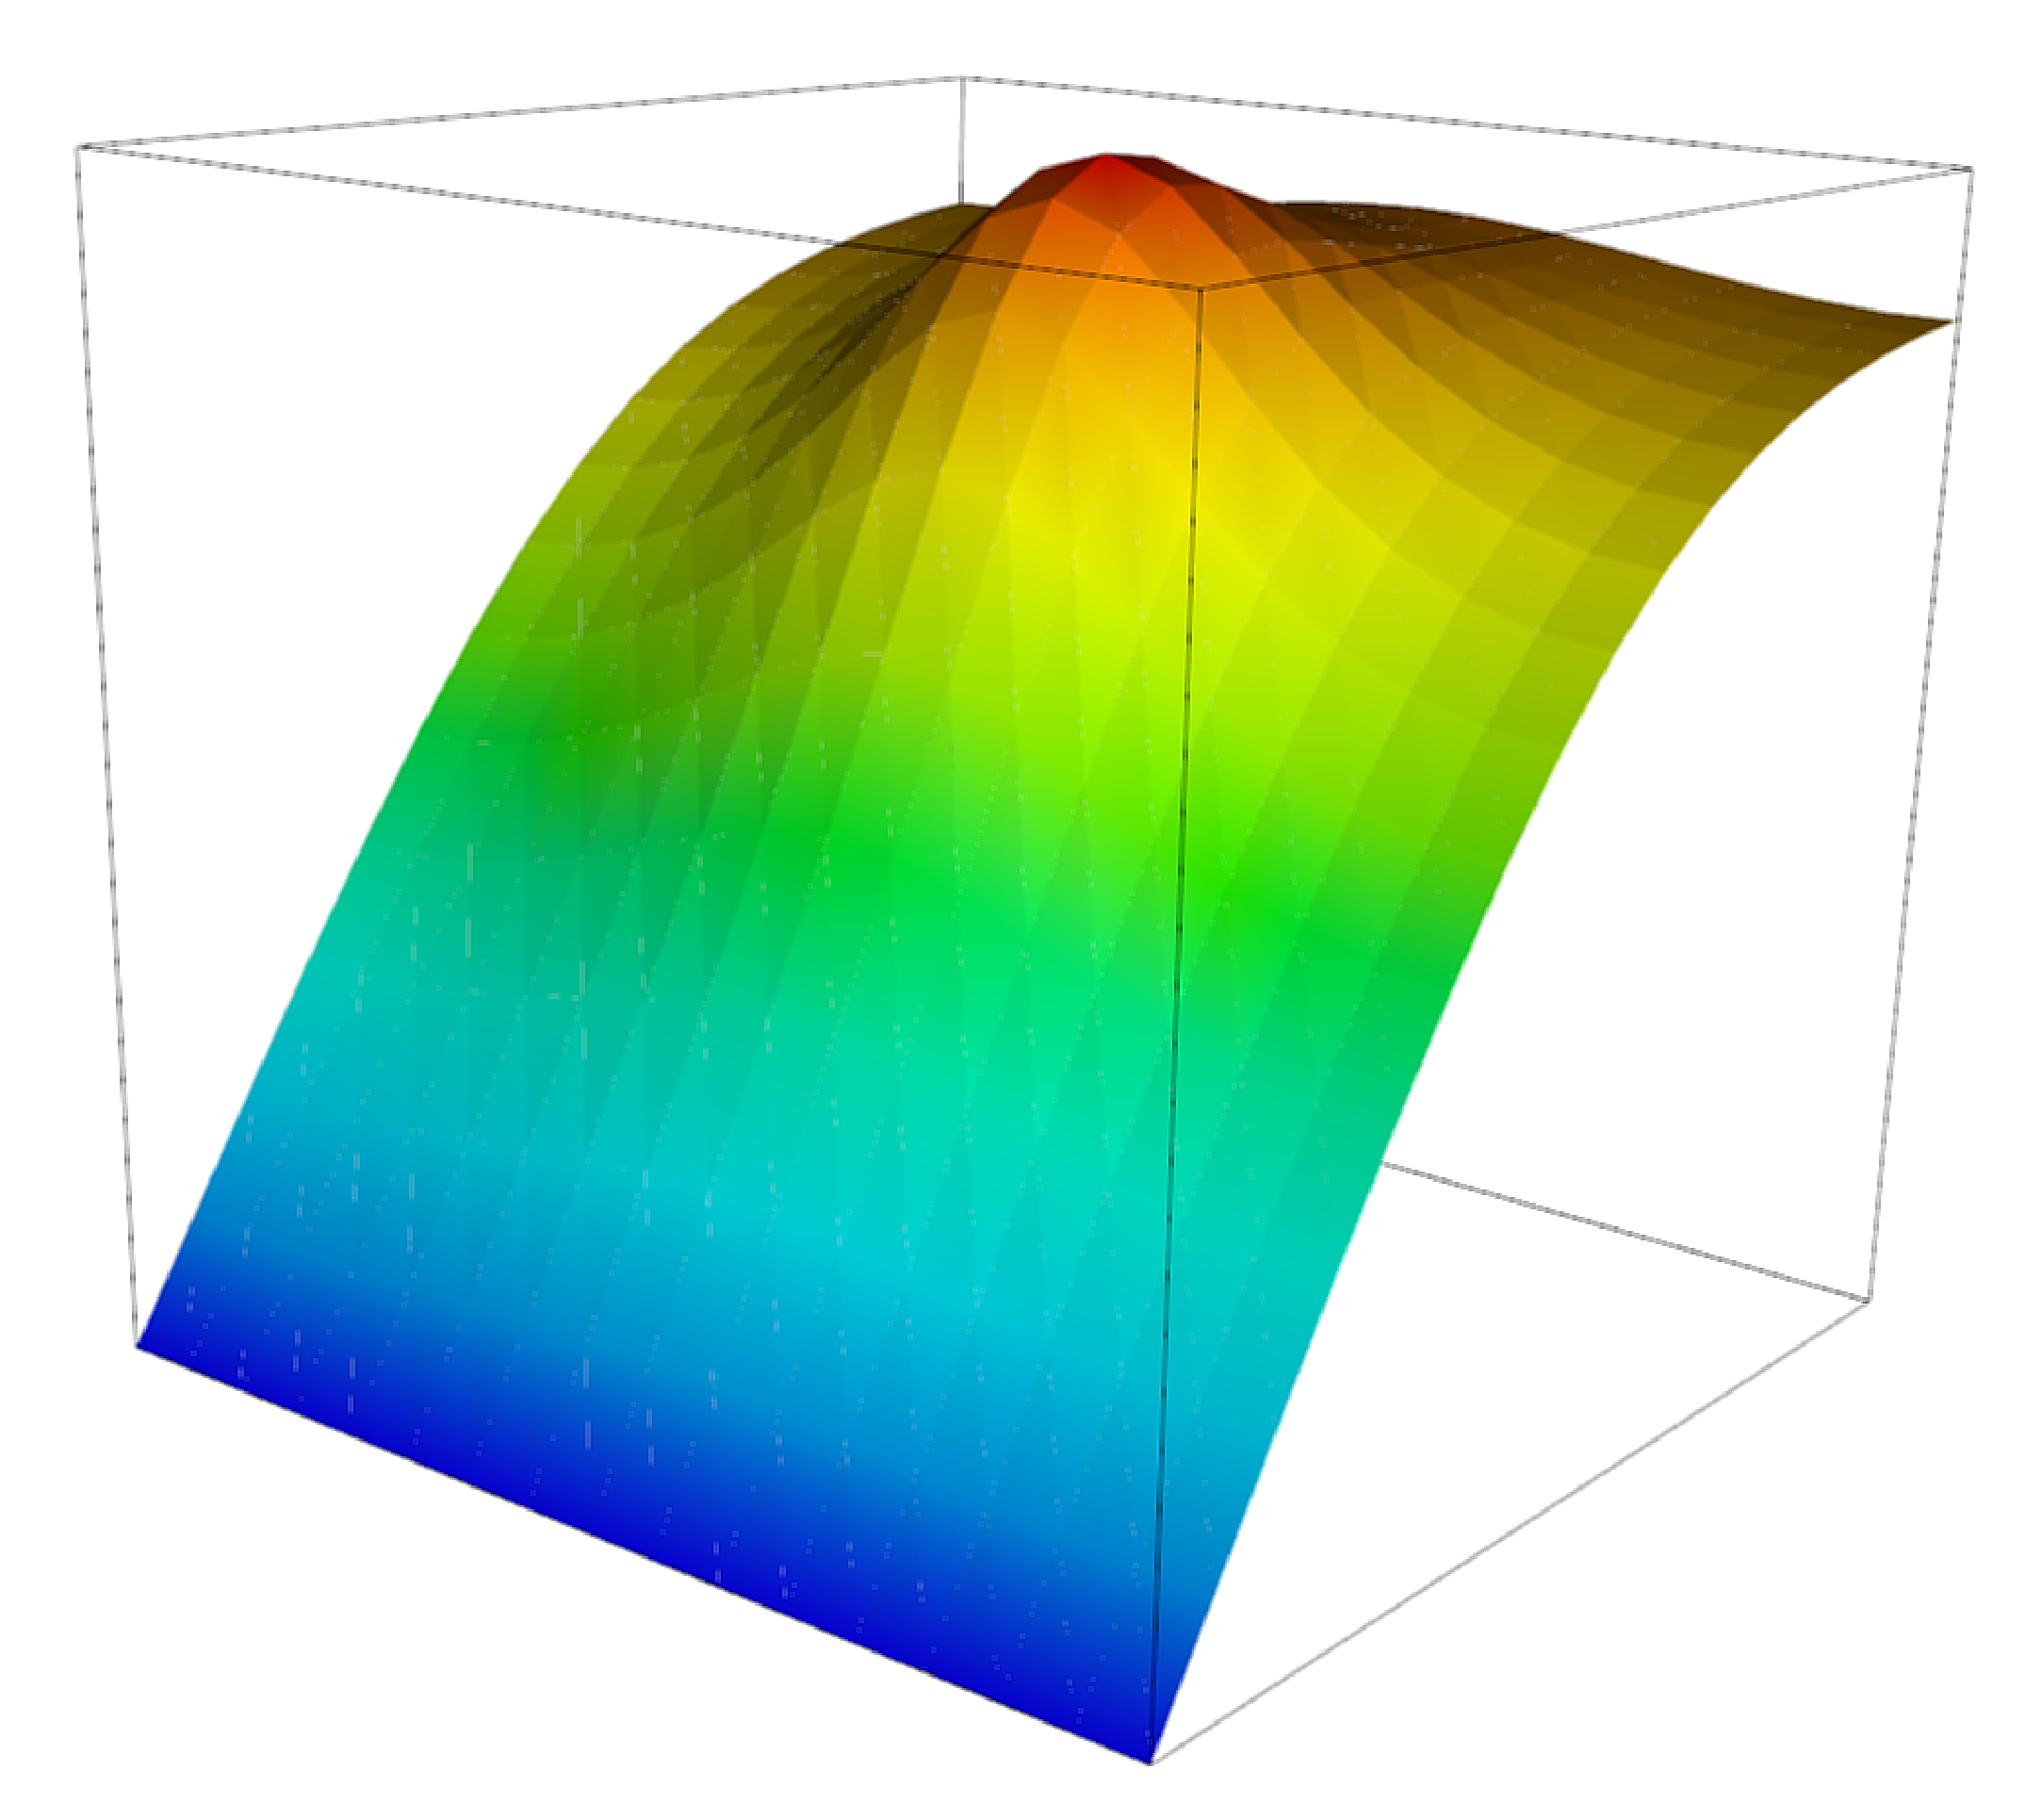
\includegraphics[width=10cm]{eps/poisson.eps}
    \caption{The solution of Poisson's equation (\ref{eq:poisson,quickstart})
      visualized in MayaVi.}
  \end{center}
\end{figure}
